\section{Approximate computing}

When architectural simplifications alone are insufficient to meet resource constraints, approximate computing techniques can be employed. 
These methods trade off some computational precision to achieve reductions in memory usage and computational load. 
Common approaches include pruning, quantization, and distillation.

A Neural Network typically consists of $l$ layers, each defined by a function $\phi_{\boldsymbol{\theta}_i}$, where $\boldsymbol{\theta}_i$ represents the parameters of the layer.
Based on this structure, two primary approximate computing techniques can be applied:
\begin{itemize}
    \item \textit{Precision scaling}: this technique reduces the memory footprint of a Convolutional Neural Network by lowering the precision of the weights.
        For instance, representing weights with fewer bits decreases memory requirements while maintaining acceptable performance.
    \item \textit{Task dropping}: this approach minimizes computational load and memory usage by selectively skipping the execution of certain tasks within the processing chain.
        These tasks may correspond to specific layers or neurons whose omission has minimal impact on the overall output quality.
\end{itemize}

\subsection{Precision scaling}
Precision scaling is achieved through quantization, which reduces the precision of weights and activations in neural networks. 
Quantization can be categorized into three main types:
\begin{itemize}
    \item \textit{Linear quantization}: this approach uses a uniform distance between quantization levels. 
        Common bit-widths include 32-bit, 16-bit, 8-bit, or custom configurations. 
        Linear quantization is widely used due to its simplicity and effectiveness.
    \item \textit{Logarithmic quantization}: the distance between quantization levels varies logarithmically. 
        When weights are powers of 2, multiplications can be replaced by efficient bit-shift operations, reducing computational complexity.
    \item \textit{Data-driven quantizer}: Quantization levels are determined or learned from the data, such as using $k$-means clustering. 
        While this approach can yield better accuracy, it introduces additional computational overhead.
\end{itemize}
\noindent Quantization can target either weights (to reduce storage requirements) or activations (typically during inference). 
Fixed quantization applies the same quantization scheme across all layers, while variable quantization tailors the quantization mechanism to specific layers, filters, or channels. 
The first and last layers of a network are often the most critical to quantize carefully, as they significantly impact accuracy.

\paragraph*{Performance}
For convolutional neural networks (CNNs), quantizing convolutional layers to 8 bits and fully connected layers to 4 bits typically results in negligible accuracy loss for weights. 
Activations, however, are usually quantized to 16 bits, as their quantization has a more pronounced impact on performance. 
Interestingly, quantization can sometimes act as a regularizer, slightly improving accuracy in rare cases.

In practice, implementing data in 8-bit formats is common.
Four 8-bit operations are approximately equivalent to one 32-bit operation within a given clock cycle.
An 8-bit fixed-point addition consumes 3.3 times less energy than a 32-bit fixed-point addition and 30 times less energy than a 32-bit floating-point addition.
An 8-bit fixed-point multiplication consumes 15.5 times less energy than a 32-bit fixed-point multiplication and 18.5 times less energy than a 32-bit floating-point multiplication.

Extreme quantization techniques push the limits of precision reduction:
\begin{itemize}
    \item \textit{Binary networks}: weights are restricted to -1 and +1 by computing the sign of the output. 
        Binary Connect uses binary weights, while Binary Neural Networks use both binary weights and activations. 
        These methods incur an accuracy loss of approximately 20\%-30\%.
    \item \textit{Ternary networks}: weights are restricted to -w, 0, and +w. 
        Ternary weight networks share the same scale factor for all weights, while trained ternary quantization learns a different scale for each weight. 
        Ternary quantization incurs minimal accuracy loss ($\approx0.5\%$) and is of theoretical interest.
\end{itemize}

\subsubsection{Implementation}
A schematic overview of matrix-multiply logic in NN accelerator hardware involves weights $w_{n,m}$ and input values $x_n$.
The Multiply-Accumulate (MAC) result is computed as:The Multiply-Accumulate (MAC) result is computed as:
\[A_n=b_n+\sum_mC_{n,m}\] 
Here, $C_{n,m}$ is the product of weight $w_{n,m}$ and input $x_n$. 
\begin{figure}[H]
    \centering
    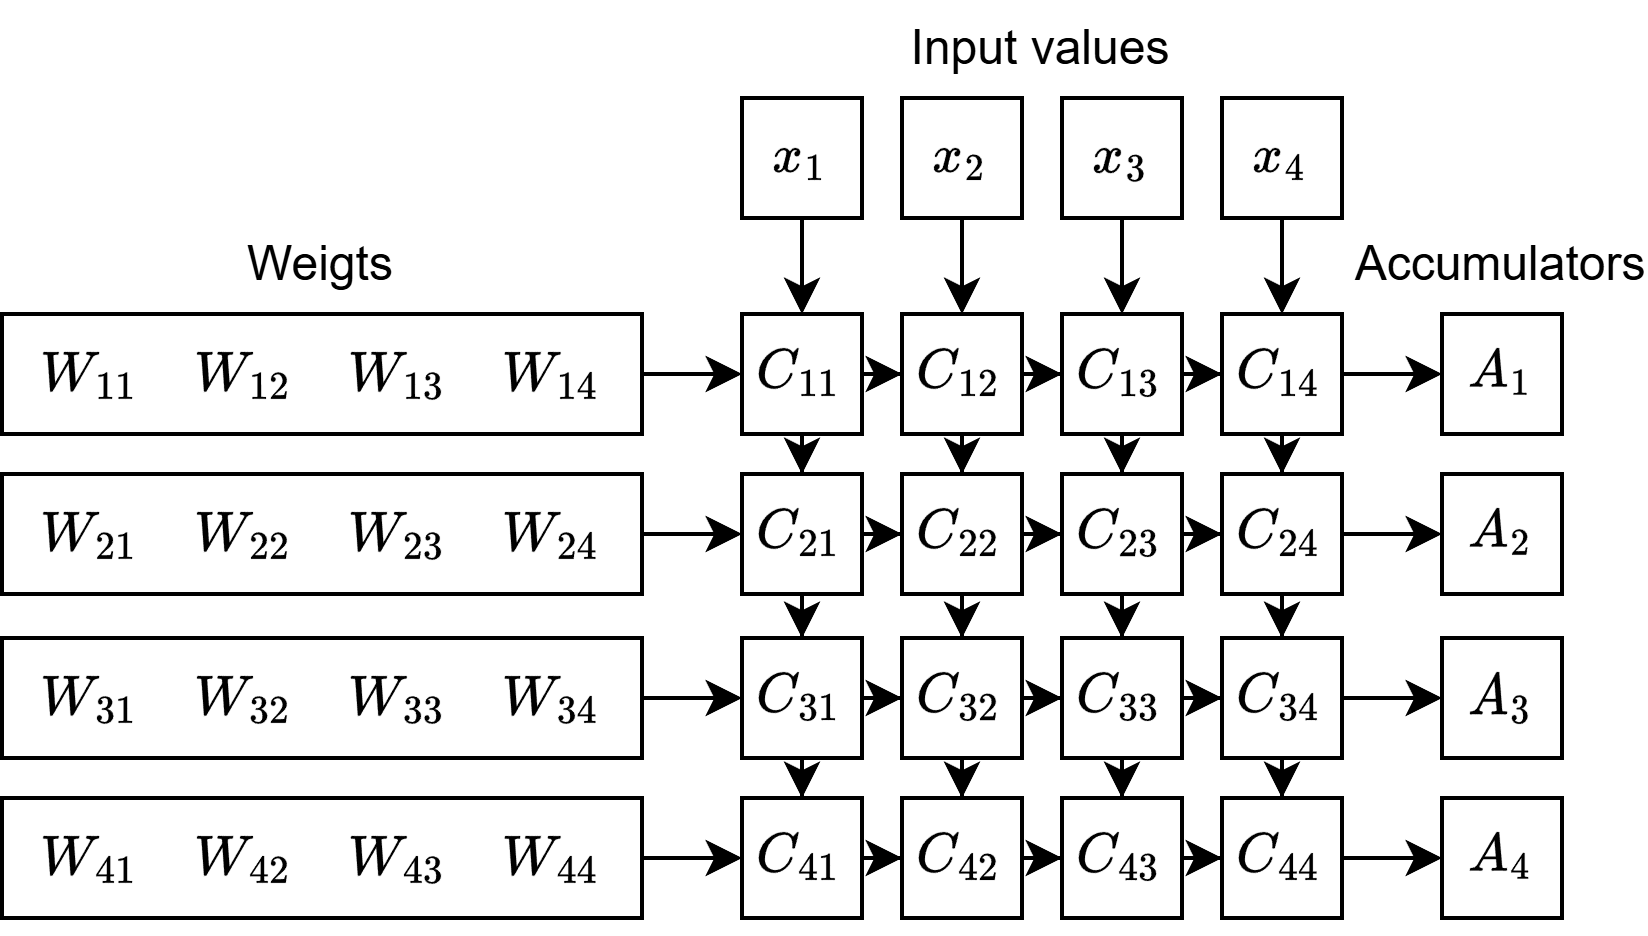
\includegraphics[width=0.75\linewidth]{images/eeai9.png}
    \caption{Schematic of MAC operation}
\end{figure}
Quantization maps floating-point values to an integer grid defined by parameters such as bit-width ($b$), scale factor ($s$), and zero-point ($z$, for asymmetric quantization).
The scale factor specifies the step size, while the zero-point ensures that real zero is quantized without error.

\paragraph*{Symmetric unsigned quantization}
For symmetric unsigned quantization (range $[0,255]$), the step size is $s$. 
A number is represented as $s\cdot x_{\text{uint8}}$, where $x_{\text{uint8}}$ is an unsigned integer. 
Quantization is performed as:
\[x_{\text{int}}=\text{clamp}\left(\left\lfloor \dfrac{x}{s}\right\rceil;0,2^{b-1} \right)\]
\noindent And de-quantization is:
\[\hat{x}=s\cdot x_{\text{int}}\]

\paragraph*{Symmetric signed quantization}
For symmetric signed quantization (range: $[-128, 127]$), the step size is $s$.
A number is represented as $s\cdot x_{\text{int8}}$, where $x_{\text{int8}}$ is an unsigned integer. 
Quantization is:
\[x_{\text{int}}=\text{clamp}\left(\left\lfloor \dfrac{x}{s}\right\rceil;-2^{b-1},2^{b-1}-1 \right)\]
\noindent And de-quantization remains:
\[\hat{x}=s\cdot x_{\text{int}}\]

\paragraph*{Asymmetric unsigned quantization}
For asymmetric quantization (range: $[-sz,255]$), the step size is $s$, and the representation is $s\cdot (x_{\text{int8}}-z)$. 
Quantization is:
\[x_{\text{int}}=\text{clamp}\left(\left\lfloor \dfrac{x}{s}\right\rceil+z;0,2^b-1 \right)\]
\noindent And de-quantization is:
\[x\approx\hat{x}=s(x_{\text{int}}-z)\]
\noindent The quantization limits are:
\[q_{\min}=-sz\qquad q_{\max}=s(2^b-1-z)\]
Values outside this range are clipped, introducing clipping errors. 
Increasing the scale factor $s$ expands the quantization range, reducing clipping errors but increasing rounding errors, which are bounded by:
\[\left[-\dfrac{1}{2}s,\dfrac{1}{2}s\right]\]
\noindent This trade-off between clipping and rounding errors must be carefully managed to achieve optimal performance.

\paragraph*{Multiply and accumulate}
A floating-point vector $\mathbf{x}$ can be approximated as a scalar multiplied by a vector of integer values.
By quantizing the weights and activations, the quantized version of the multiply-and-accumulate (MAC) operation is expressed as:
\[\hat{A}_n=\hat{\textbf{b}}_n+s_{\textbf{w}}s_{\textbf{x}}\sum_m\textbf{W}_{n,m}^{\text{int}}\textbf{x}_m^{\text{int}}\]
Here, $s_{\textbf{w}}$ and $s_{\textbf{x}}$ are scale factors for weights and activations, respectively. 
This formulation separates the scale factors, enabling efficient computation while maintaining precision.

\subsubsection{Usage}
Quantization reduces the computational cost and memory footprint of neural networks by converting floating-point representations into fixed-point representations. 
Two primary approaches exist: post-training quantization (PTQ) and quantization-aware training (QAT).

\paragraph*{Post-Training Quantization}
In PTQ, a pre-trained floating-point (FP32) network is directly converted into a fixed-point network without requiring retraining or access to the original training pipeline. 
The main challenge lies in determining the appropriate quantization range settings. 
Common methods include MinMax quantization and Mean Squared Error (MSE) optimization.
MinMax quantization sets the range based on the minimum and maximum values of the tensor:
\[q_{\min}=\min\mathbf{V} \qquad q_{\max}=\max\mathbf{V}\]
MSE optimization minimizes the difference between the original and quantized tensors:
\[\argmin_{q_{\min},q_{\max}}={\left\lVert \mathbf{V}-\hat{\mathbf{V}}(q_{\min},q_{\max})\right\rVert}_F^2 \]
PTQ is effective and fast to implement but struggles with low-bit quantization (e.g., 4-bit or below), where large quantization errors may degrade performance.

\paragraph*{Quantization-Aware Training}
QAT integrates quantization into the training process by simulating its effects during backpropagation. 
While this approach achieves higher accuracy, it requires longer training times and labeled data. 
A key challenge is handling the non-differentiability introduced by quantization. 
This is addressed using the straight-through estimator (STE), which approximates the gradient of the rounding operator as 1:
\[\dfrac{\partial\left\lfloor y\right\rceil}{\partial y}=1\]
During the forward pass, quantization is applied, while the backward pass uses un-quantized values for gradient computation. 
QAT generally outperforms PTQ, especially for low-bit quantization, but at the cost of increased complexity.
\begin{figure}[H]
    \centering
    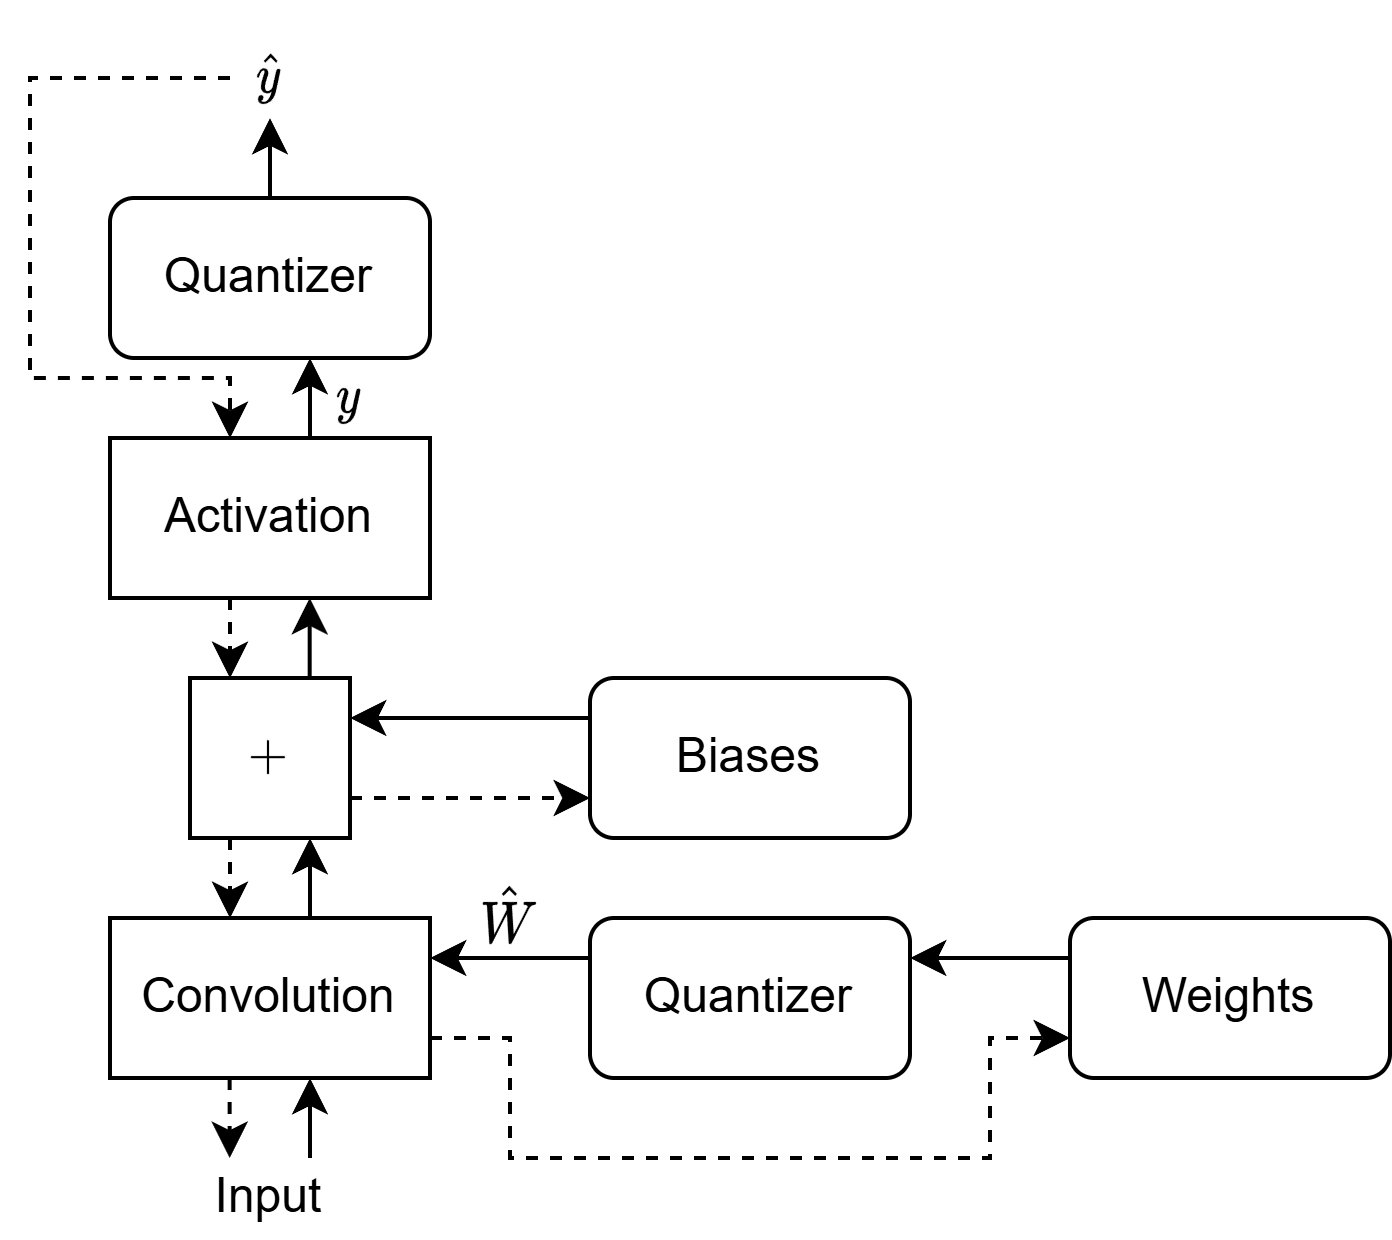
\includegraphics[width=0.75\linewidth]{images/eeai10.png}
    \caption{QAT forward and backward propagation}
\end{figure}

It is important to note that the best quantized network is not necessarily obtained by simply quantizing the best FP32 network. 
Careful optimization is required to balance accuracy and efficiency.


\subsection{Task dropping}
Reducing the number of operations and model size improves computational efficiency and memory usage. 
Several techniques achieve this goal, including:
\begin{itemize}
    \item \textit{Network pruning}: neural networks are often over-parameterized, meaning many weights are redundant and can be pruned (set to zero) without significantly affecting performance. 
        Simple pruning removes individual weights, while structured pruning removes groups of weights, such as entire rows, columns, or filters. 
        Aggressive pruning may require fine-tuning to recover accuracy.
    \item \textit{Network architecture design}: efficient architectures replace large filters with smaller ones, reducing the total number of weights. 
        Smaller filters can be concatenated before training to emulate larger ones, or tensor decomposition techniques can be applied after training to decompose filters without impacting accuracy.
    \item \textit{Transfer learning}: transfer learning leverages pre-trained models by retaining the first few layers, which capture general features, and replacing the later layers with a simpler architecture tailored to the target task. 
        This approach reduces the need for extensive retraining.
    \item \textit{Knowledge distillation}: a smaller student network learns to mimic the behavior of a larger teacher network. 
        The loss function minimizes the difference between the outputs of the two models, enabling the student to approximate the teacher's performance with fewer parameters.
\end{itemize}